 


\documentclass[a4paper,headsepline,bibliography=totoc,listof=totoc]{scrartcl}							%dokumentenklasse
\usepackage[utf8]{inputenc}															%europäische umlaute und schriftzeichen

\usepackage[table]{xcolor} 
\usepackage{adjustbox}
\usepackage{graphicx}
\usepackage{csvsimple}
\usepackage[T1]{fontenc}															%
\usepackage[ngerman]{babel}															%sprachpaket deutsch, neue deutsche rechtschreibung
  \addto\captionsngerman{%
    \renewcommand{\figurename}{Abb.}%
    \renewcommand{\tablename}{Tab.}%
  }
\usepackage{graphicx}																%png grafiken
\usepackage{svg}
\setsvg{inkscape=inkscape -z -D,svgpath=fig/}

\usepackage{listings}																%source code einbindung
%\usepackage{lmodern}																%font
%\usepackage[eso-foot]{svninfo}														%svn infos 		 
\usepackage{scrpage2}																%kopf und fußzeilen				
\usepackage{url}			
														%URL in Großbuchstaben
%\usepackage{ulem}																	%doppelt unterstreichen
%\usepackage{tikz}																	%zeichnen
%\bibliography{quellen}																%lade literatur verzeichnis
\usepackage{here}																	%exaktes plazieren der Grafiken (große PAP'S)
%\addtokomafont{sectioning}{\rmfamily}												%Titel anders gesetzt (serifenlos)
\usepackage{dirtree} 																%Dateistruktur erstellen
%\usepackage{booktabs}																%saubere Tabellen
%\usepackage{pdfpages}																%pdf direkt einbinden
%\usepackage{pgf,tikz}
%\usetikzlibrary{arrows}
%\usepackage{eurosans}
%
\usepackage{pdfpages}
\usepackage{textcomp} 

\newcommand{\degre}{\ensuremath{^\circ}}
\usepackage{wrapfig} 

\usepackage{amsmath}
 
\usepackage[
        colorlinks=false,
        pdfborder={0 0 0},
	    pdftitle={Projektdokumentation KlausurNoten App},
	    pdfsubject={Dokumentation der Durchführung der Android Projektarbeit unter Leitung von Prof. Dr. Karlheinz Blankenbach},
	    pdfauthor={Julian Wiche},
	    pdfkeywords={Android, Projektarbeit, KlausurNoten}
	]{hyperref}


%\usepackage{europs} 
%****************************************************************************************************************************************************
%anpassungen für listings 
\usepackage{color}
\definecolor{mygreen}{rgb}{0,0.6,0}
\definecolor{mygray}{rgb}{0.5,0.5,0.5}
\definecolor{mymauve}{rgb}{0.58,0,0.82}
\definecolor{ffqqtt}{rgb}{1,0,0.2}
\definecolor{qqzzqq}{rgb}{0,0.6,0}
\definecolor{qqqqff}{rgb}{0,0,1}




\lstset{ %
   backgroundcolor=\color{white},   % choose the background color; you must add \usepackage{color} or \usepackage{xcolor}
   basicstyle=\footnotesize,        % the size of the fonts that are used for the code
   breakatwhitespace=false,         % sets if automatic breaks should only happen at whitespace
   breaklines=true,                 % sets automatic line breaking
   captionpos=b,                    % sets the caption-position to bottom
   commentstyle=\color{mygreen},    % comment style
   deletekeywords={...},            % if you want to delete keywords from the given language
   escapeinside={\%*}{*)},          % if you want to add LaTeX within your code
   extendedchars=true,              % lets you use non-ASCII characters; for 8-bits encodings only, does not work with UTF-8
   frame=single,                    % adds a frame around the code
   keepspaces=true,                 % keeps spaces in text, useful for keeping indentation of code (possibly needs columns=flexible)
   keywordstyle=\color{blue},       % keyword style
   language=Matlab,                 % the language of the code
   morekeywords={byte},            % if you want to add more keywords to the set
   numbers=left,                    % where to put the line-numbers; possible values are (none, left, right)
   numbersep=5pt,                   % how far the line-numbers are from the code
   numberstyle=\tiny\color{mygray}, % the style that is used for the line-numbers
   rulecolor=\color{black},         % if not set, the frame-color may be changed on line-breaks within not-black text (e.g. comments (green here))
   showspaces=false,                % show spaces everywhere adding particular underscores; it overrides 'showstringspaces'
   showstringspaces=false,          % underline spaces within strings only
   showtabs=false,                  % show tabs within strings adding particular underscores
   stepnumber=1,                    % the step between two line-numbers. If it's 1, each line will be numbered
   stringstyle=\color{mymauve},     % string literal style
   tabsize=2,                       % sets default tabsize to 2 spaces
   %float=hbt,
   title=\lstname,                   % show the filename of files included with \lstinputlisting; also try caption instead of title
   escapeinside={(*@}{@*)}			%labels im listing
}

\setlength{\parindent}{0pt}

\lstdefinelanguage{HTML5}{
        language=html,
        sensitive=true, 
        alsoletter={<>=-},
        otherkeywords={
        % HTML tags
        <html>, <head>, <title>, </title>, <meta, />, </head>, <body>,
        <canvas, \/canvas>, <script>, </script>, </body>, </html>, <!, html>, <style>, </style>, ><
        },  
        ndkeywords={
        % General
        =,
        % HTML attributes
        charset=, id=, width=, height=,
        % CSS properties
        border:, transform:, -moz-transform:, transition-duration:, transition-property:, transition-timing-function:
        },  
        morecomment=[s]{<!--}{-->},
        tag=[s]
}

\lstdefinestyle{phpnocomment}
{
    numberblanklines=false,
    language=php,
    tabsize=4,
    commentstyle=\color{white},
    keywordstyle=\color{red}
    %identifierstyle= %plain identifiers for make
}


%****************************************************************************************************************************************************

\begin{document}
\pagestyle{headings}

\begin{titlepage}
\begin{center}


\includegraphics[width=0.9\textwidth]{./img/logo} \\[0.8 cm]

\text{\LARGE \textbf{Fakultät für Technik}}\\[0.3 cm]

\text{\LARGE \textbf{Bereich Informationstechnik}}\\[0.3 cm]

\text{ }

\text{\LARGE \textbf{Bachelorthesis}}\\[1.5 cm]

\text{Thema:}\\[1 cm]

\text{\Large\textbf{SPS- Kleinsteuerung mittels Rasperry Pi}}\\[0.5 cm]

\text{Konzept und Implementierung einer SPS- Kleinsteuerung auf einem }\\
\text{Raspberry Pi mit graphischer Programmierung und IFTTT-funktionalität }\\[1 cm]

\begin{tabular}[h]{ll}

 \textbf{Betreuer} &Prof. Dr. Karlheinz Blankenbach \\&Prof. Dr.-Ing. Thomas Greiner\\[0.3 cm] 


 \textbf{vorgelegt von:} &  Julian Wiche\\ 
 & Matrikelnummer: 306675\\[0.3 cm] 

 \textbf{Abgabetermin} & 19.05.2019 \\[0.3 cm] 

 

\end{tabular} 

\end{center}
\end{titlepage}


\tableofcontents
																%inhaltsverzeichnis
\setcounter{page}{1}
\newpage

%------------------------------------------------ %

\lstset{literate=%
    {Ö}{{\"O}}1
    {Ä}{{\"A}}1
    {Ü}{{\"U}}1
   %    {ß}{{\ss}}1
    {ü}{{\"u}}1
    {ä}{{\"a}}1
    {ö}{{\"o}}1
    {~}{{\textasciitilde}}1
}

\newcommand{\hex}{\textsubscript{h} }

\newcommand{\gqq}[1]{\glqq{}#1\grqq{}}
\newcommand{\gq}[1]{\glq{}#1\grq{}}
\newcommand{\fqq}[1]{\flqq{}#1\frqq{}}

\newcommand{\chphl}[1]{\textit{\frqq{}#1\flqq{}}}




\newcommand{\pthPhpScripts}{../serial2DB}
\newcommand{\pthWeb}{../Webinterface}

%setting paths for chapters
\newcommand{\pthChps}{chp}
\newcommand{\pthImg}{img}
\newcommand{\pthDoc}{doc}





%\newcommand{\pthEinleitung}{\pthChps/einleitung}
%\section{Einleitung}
%\label{chp:Einleitung}
% \section{Einleitung}
 Speicherprogrammierbare Steuerungen oder kurz SPS tauchen überall dort auf, wo große elektrische Maschinen eingesetzt werden. Dies ist vor allem in der Industrie der Fall. Ihr kleiner Bruder ist die Kleinsteuerung. Sie bietet die selben Kernfunktionen, hat jedoch eine deutlich kleinere Anzahl an Ein- und Ausgängen. Sie werden häufig von Elektroinstallateuren eingesetzt, wenn eine klassische Verbindungsprogrammierte Steuerung zum Beispiel durch Drahtbruch oder defekte Spulen in eingesetzten Relais nicht mehr korrekt funktionieren. Der Hersteller Eaton hat mit seinem Produkt \chphl{Easy} genau diese Zielgruppe im Blick. Die Programmierung erfolgt hier, als würde man klassische Schütz-Kontakte in Reihe schalten. Die Einstiegsgeräte sind relativ preiswert, doch kauft man sich in eine proprietäre Produktwelt ein, welche aufgrund von inkompatiblen Bauteilen und Bussystemen schwer wieder zu verlassen ist. So gestaltet sich die Erweiterung einer bestehenden Steuerung um die Möglichkeit einer Fernabfrage übers Internet als nahezu unmöglich, oder setzt den Austausch der kompletten Steuerung voraus. Dabei sind Ein- und Ausgänge doch eigentlich das selbe wie an jedem Raspberry Pi vorhandene GPIOs. Auf Basis dieser Überlegung und günstigen Preisen hierfür, entstand die Idee eine Lösung mittels Raspberry Pi zu erarbeiten. 
\subsection{Ziel der Arbeit}
Ziel dieser Arbeit ist es dabei vor allem eine möglichst günstige Möglichkeit zu schaffen um eine Steuerung zu realisieren, welche intuitiv programmiert werden kann und die Grundsätzliche Funktion der vorher eingesetzten Easy Steuerung um Funktionen zur Fernabfrage übers Internet und weitere Funktionen erweitert. Dabei soll das Projekt mittels Git versioniert werden um es anderen Entwicklern auf GitHub als Open-Source Software zur Verfügung zu stellen. Dabei wird das Projekt als MIT Lizensiert, was eine Modifikation sowie private und gewerbliche Nutzung und Verbreitung ausdrücklich gestattet. 
\subsection{Verwandte Arbeiten}
Weitere Projekte mit denen ähnliches möglich ist, sind hierbei das Kommerzielle Projekt Codesys *REF*. Auch zu nennen ist das Projekt Open-PLC *REF*   
\subsection{Aufbau der Arbeit}
\todo{ Aufbau der Arbeit fertigstellen}
\clearpage

%\newpage
%
%
%\newcommand{\pthAnalyse}{\pthChps/analyse}
%\section{Analyse des Messsystems}
%\label{chp:Analyse}
%\input{\pthAnalyse/analyse.tex}
%
%
%\newcommand{\pthAuswertung}{\pthChps/auswertung}
%\section{Datenerfassung und Speicherung}
%\label{chp:Auswertung}
%\section{Übersicht Gesamtsystem}\label{kap:ausw}
 \subsection{Inbetriebnahme}
 \subsubsection{Hardware Voraussetzungen}
 Voraussetzung für den Betrieb ist ein Raspberry Pi 2 oder 3. Außerdem ist eine Erweiterungsplatine \chphl{PiFace Digital2 \cite{URL:PiFaceDigital2}} erforderlich. Diese muss vor dem ersten Start auf die GPIO-Kontakte des Raspberry Pi aufgesteckt werden. Eine Funktion ohne das Hardwaremodul ist Grundsätzlich möglich, jedoch scheint ein Betrieb ohne Hardwareschnittstelle ohne Sinn. Die Software ist so konzipiert, dass auch andere Hardware-Module denkbar sind, eine Implementierung hierfür fehlt jedoch bislang.     
 \subsubsection{Software Voraussetzungen}
 Für den Betrieb wird ein Linux Betriebssystem vorausgesetzt. Hierfür kann das angepasstes Raspbian \cite{URL:Raspian} Image genutzt werden, welches auf der beigelegten DVD zu finden. Falls auf der SD Karte bereits ein Linux Betriebssystem installiert ist, kann das Arbeitsverzeichnis des Projekts auch einfach auf den Raspberry Pi übertragen werden. Ein Git Auszug hiervon ist ebenfalls auf der beigelegten DVD. Sollte die Wahl der Distribution auf eine andere als Raspbian Strech \cite{URL:Raspian} fallen, so muss das Projekt aus den Quellen übersetzt werden. In jedem Fall ist es nötig dass SPI aktiviert wird. Dies geschieht am einfachsten über das Raspberry Pi Konfigurationsprogramm.  \texttt{sudo raspi-config} siehe \cite{URL:EnableSPI}.  
 \subsubsection{Kompilieren des Projekts}
 Ein kompilieren des Projekts ist nur erforderlich, wenn das Projekt auf einem anderen Betriebssystem als Raspbian Strech \cite{URL:Raspian} verwendet werden soll, oder wenn Änderungen am Quellcode vorgenommen werden sollen. Dafür muss zunächst eine SSH Verbindung zum System herstellt werden. Das Projekt sollte daraufhin auf das System übertragen werden. Die empfohlene Vorgehensweise hierfür ist, das GIT Repository über eine aktive Internetverbindung auf den Rasperry Pi zu klonen. \texttt{git clone https://github.com/dajuly20/ControlPi}. Um dann alle Abhängigkeiten automatisch zu installieren, kann das nachfolgend genannte Installationsscript verwendet werden: \texttt{./start\_pull\_and\_build.sh}. Sollte keine Internetverbindung bestehen, können die auf der DVD mitgelieferten Bibliotheken auch manuell installiert werden. 
 Eine Liste der benötigen Abhängigkeiten findet sich im \nameref{chp:anhang} in \autoref{chp:anhang}.  
 \subsubsection{Inbetriebnahme unter Raspbian Strech}
 Sollte auf dem Raspberry Pi bereits ein Version von Raspbian in der Version Strech installiert sein, so genügt es den Projektordner auf den Raspberry Pi zu übertragen. Hierfür dient entweder der Ordner \texttt{ControlPi} auf der beigelegten DVD, oder das GIT Repository des Projekts, welches mittels  \texttt{git clone https://github.com/dajuly20/ControlPi} auf den Raspberry Pi übertragen werden kann. Um sicherzustellen dass es sich um die aktuellste Version handelt, sollte das Projekt mit \texttt{git pull} auf den neusten Stand gebracht werden. Daraufhin kann mit \texttt{./start\_manual.sh} die Funktion überprüft werden. Dabei sollte der Benutzer in den Gruppen \texttt{spi} sowie \texttt{gpio} sein. Letztlich sollte das Projekt als Systemservice eingerichtet werden. Hierfür ist das Script \texttt{./start\_as\_service.sh} dienlich. Es wird hier neben dem eigenen Systemservice auch ein Apache2 Webserver mit in Betrieb genommen.
 
 \subsection{Inbetriebnahme mit Systemabbild}
 Auch befindet sich ein vollständiges Systemabbild \cite{URL:Image} auf der beigelegten DVD. Dieses sollte zunächst mit \texttt{tar -xvzf ControlPi-Raspbian-Strech.tar.gz} entpackt werden. Die enthaltene \texttt{.img} Datei belegt ca. 7,3 GB. Eine Speicherkarte sollte also mindestens 8 GB besser jedoch 16 GB Platz bieten. Das Systemabbild kann mit \texttt{sudo dd if=ControlPi-Raspbian-Strech.img of=/dev/<XXX> bs=4M status=progress}, oder unter Windows mit einem entsprechenden Tool \cite{URL:Win32DiskImager} auf eine Speicherkarte übertragen werden. Nach erfolgreichem Start sollte eine der LEDs auf der PiFace Erweiterungskarte dauerhaft blinken.  
 
 \subsubsection{Ermittlung der IP - Adresse}\label{chp:ausw:ip}
 Nachdem der Systemservice läuft, muss nun ermittelt werden wie ein Zugriff auf die Weboberfläche erfolgen kann. Wenn der Raspberry Pi in ein bestehendes Netzwerk integriert wird, kann dies in der Oberfläche des verwendeten Internetrouters nachgesehen werden. Sofern dieser dies unterstützt, kann auch der Hostname des Raspberry Pi für den Zugriff verwendet werden. Der Hostname im mitgelieferten Raspbian-Image lautet \texttt{ControlPi3}. Der Standard bei einem offiziellen Raspbian Image ist \texttt{raspberrypi}. Sollte kein Zugriff auf den Internetrouter bestehen oder eine Ermittlung der IP Adresse aus sonstigen gründen nicht möglich ist, kann ein Portscan durchgeführt werden. Die Steuerung öffnet in der Standartkonfiguration die Ports 80 für HTTP, den Port 443 für HTTPS bzw. SSL und den Port 22 für SSH Zugriffe. Angenommen eigene IP Adresse (Ermittlung durch \texttt{ifconfig}) wäre 192.168.8.5 mit der Subnetzmaske 255.255.255.0 so wäre der Aufruf \texttt{nmap -p 22,80,443 192.168.8.0/24}. Sollten mehrere gefundene Geräte diese Ports als offen anzeigen, so sollten die IP Adressen dieser Geräte nacheinander im Webbrowser als URL eingetragen werden um zu überprüfen bei welcher es sich um die richtige handelt.   
 
 \subsection{Funktionstest}
 \subsubsection{Testen der Betriebsbereitschaft}
 Im Auslieferungszustand ist ein zu Testzwecken bereits ein Steuerungsprogramm enthalten. Dieses lässt die LED an Ausgang 6 durch einen sich selbst aufrufenden Timer blinken. Zudem ist in diesem Testprogramm den Ausgängen \texttt{0} sowie \texttt{1} der Wert der Eingänge \texttt{0} beziehungsweise \texttt{1} zugewiesen. Ein Drücken der in \autoref{img:PiFaceDigital2} gezeigten Taster S0 oder S1 sollte also ein Leuten der entsprechenden LED zur Folge haben. Wie auch bei den Tastern, werden die LEDs von rechts nach links durchnummeriert und sind den jeweiligen Ausgängen örtlich zugeordnet. Da an den Ausgängen \texttt{0} und \texttt{1} zudem Relais angeschaltet sind, sollte sich ein Zustandswechsel auf einem dieser Ausgängen außerdem in Form eines Klickgeräusches akustisch bemerkbar machen. 

 
 \begin{figure}[H]
 	\begin{center}
 		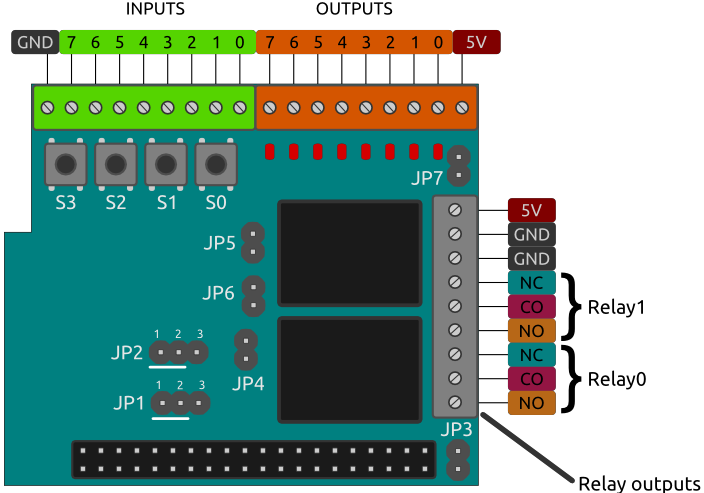
\includegraphics[width=0.95\textwidth]{./images/pifacedigital2_diagram.png}
 		\caption[Darstellung eines PiFace Digital 2]{Darstellung eines PiFace Digital 2 \cite{URL:Pfd}}
 		\label{img:PiFaceDigital2}
 	\end{center} 
 \end{figure}	

 \subsubsection{Aufruf der Weboberfläche}\label{chp:FrontendUebersicht}
Ist der Hostname oder die IP Adresse des Raspberry Pi ermittelt (siehe Abschnitt \ref{chp:ausw:ip} \nameref{chp:ausw:ip}), kann dieser im Internetbrowser aufgerufen werden. Bei Verwendung des beigelegten Raspbian Images wäre der Aufruf \texttt{http://ControlPi3}. \autoref{img:FrontendUebersicht} zeigt die Übersichtsseite der Steuerung. In der Mitte befindet sich eine Abbildung vom aktuell verwendeten Steuerungsprogramm, während an den Seiten die Zustände ein und Ausgänge angezeigt werden. Die Drop-Down Menüs oberhalb, ermöglichen es die gewünschte Ein- bzw. Ausgangsentität auszuwählen. Handelt es sich bei der ausgewählten Entität um einen Eingang, so wird anstelle einer LED ein Taste eingeblendet. Der Zustand kann dann, bei entsprechender Berechtigung (siehe \chpref{chp:ums:websock:auth} ), durch anklicken verändert werden.  

 \begin{figure}[H]
	\begin{center}
		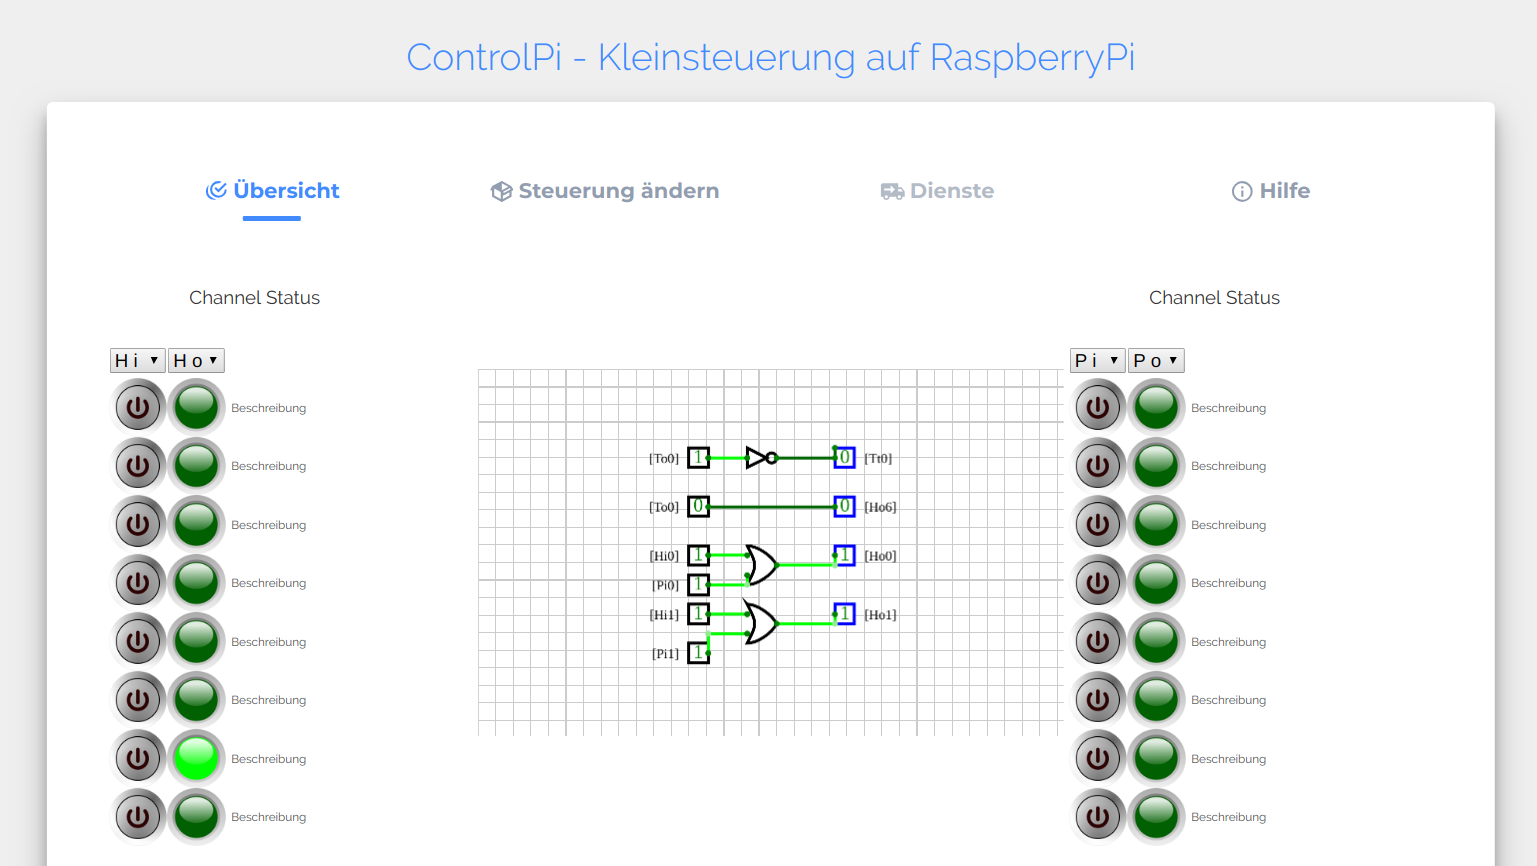
\includegraphics[width=0.95\textwidth]{./images/FrontendUebersicht.png}
		\caption{Darstellung Frontend Übersicht}
		\label{img:FrontendUebersicht}
	\end{center} 
\end{figure}

\subsubsection{Erstellen eines Steuerungsprogramms}

Um ein Steuerungsprogramm zu erstellen, muss zunächst der Tab \texttt{Steuerung ändern} angewählt werden. Nun erscheint der in \autoref{img:FrontendAenderung} abgebildete Logik-Editor CicuitVerse \cite{URL:CircuitVerse}. Sollte die vorhandene Logikschaltung nicht sofort sichtbar sein, muss die Zeichenfläche zuerst durch klicken auf das Fadenkreuz-Symbol in den Mittelpunkt gerückt werden. Soll nun eine komplett neue Schaltung gezeichnet werden, kann die Zeichenfläche durch den Unterpunkt \texttt{Clear Project} im Drop-Down Menü \texttt{Project} bereinigt werden. Alle verfügbaren Bauteile befinden sich im Bauteil-Menü auf der linken Seite. Dieses ist in die Kategorien \texttt{Input} \texttt{Output} und \texttt{Gates} unterteilt, welche sich durch anklicken aufklappen lassen. Möchte man ein Bauteil auf die Zeichenfläche schieben, so muss dieses angeklickt und der Cursor auf die Zeichenfläche bewegt werden. Ein erneutes Klicken lässt das Bauteil an der gewählten Position fallen. Die Bauteile werden schließlich mittels Drag \& Drop mit einander Verbunden. Werden Timerbausteine angeklickt, so  lassen  sich dessen Einschalt und Ausschalt- Verzögerungszeiten im Menü \texttt{Properties} einstellen. Es gilt zu beachten, dass Ausgänge jeweils nur einmal vorkommen dürfen. Gibt es mehrere Möglichkeiten in denen ein Ausgang aktiv werden soll, empfiehlt sich die Verwendung eines Und- bzw. Oder- Gatters. Nach Vollendung des Steuerungsprogramms, kann die Steuerung mit dem Menüpunkt \texttt{Save \& Export}, welcher sich im Menü \texttt{Project} befindet, übernommen und getestet werden. Eine Überprüfung auf Richtigkeit des Steuerungsprogramms erfolgt nicht. Deshalb sollte der Info-Kasten \texttt{Backend Status} im Auge behalten werden. Falls ein Fehler mit dem Steuerungsprogramm auftritt, wird dieser dort angezeigt. 
	

 \begin{figure}[H]
	\begin{center}
		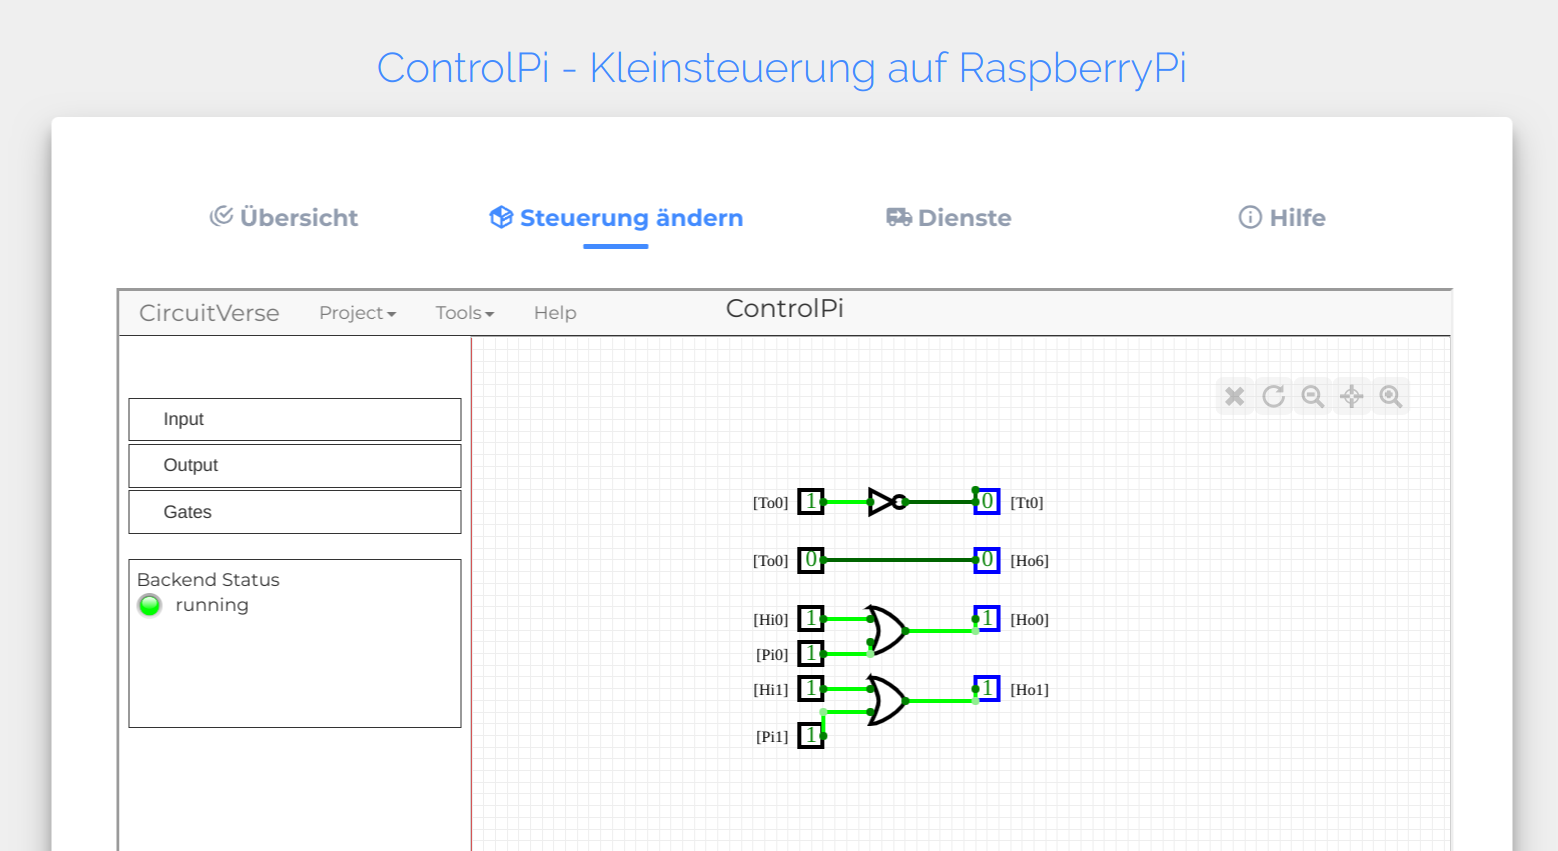
\includegraphics[width=0.95\textwidth]{./images/FrontendAendern.png}
		\caption{Darstellung Logik Editor}
		\label{img:FrontendAenderung}
	\end{center} 
\end{figure}	

\subsection{Langzeittest}
Um zu Testen wie sich die Steuerung längerfristig verhält wurde ein Timerbaustein verwendet, welcher sich selbst nach Ablauf schaltet und somit oszilliert. Als Testzeitraum wurde 48 Stunden gewählt. Dabei ließ sich feststellen, dass die Steuerung auch nach Ablauf dieser Zeit ohne Fehler weiterhin blinkte. Eine Recherche nach Neustarts des Systemdienstes blieb ebenfalls ohne Treffer.    

 \subsection{Bugs}
 Zum derzeitigen Stand sind noch einige Probleme enthalten auf die nachfolgend eingegangen wird. Als erstes sei hier zu nennen, dass die Reihenfolge in welcher das Backend über die Zeilen des erzeugten Steuerungsprogramms Iteriert unter bestimmten Voraussetzung Probleme bereitet. So wird der Wert eines Ausgangs unter noch nicht näher bekannten Umständen erst mit der nächsten Iteration des Logikprogramms übernommen. Dies könnte durch generelles doppeltes iterieren behoben werden, was allerdings die Performance vermindert. Der Logikeditor in der Benutzeroberfläche hat ebenfalls ein Darstellungsproblem welches bislang noch nicht behoben werden konnte. Beim Aufruf wird die bereits vorhandene Logikschaltung nicht Automatisch zentriert, sondern ist beinahe unsichtbar in der oberen linken Ecke der Zeichenfläche. Ein klicken auf das Fadenkreuz-Symbol bringt hier Abhilfe.  
 
 \subsection{Fazit}
 Das Projekt teilte sich wesentlich in zwei Teile. Das Backend ist einen Teil, welcher sich auf einer sehr Hardwarenahen Ebene abspielte. Die Benutzeroberfläche hingegen, ist sehr nahe am Benutzer. Damit spiegelte dieses Projekt viele Nuancen der Technischen Informatik wieder. Die meiste Arbeit entfiel dabei in die Programmierung des Backend, dass in mehrere parallele Handlungsstränge aufgeteilt ist, welche synchronisiert werden wollen. Auch das arbeiten mit C++ Bibliotheken und das Kompilieren brachte einige Herausforderungen mit sich. Die Anbindung der Benutzeroberfläche beleuchteten eine relativ junge Technologie der modernen Webentwicklung. Auch das Anpassen des Logik Editors und die damit verbundene Einarbeitung in ein fremdes Open-Source Projekt machten dieses Projekt sehr lehrreich. Zuletzt boten sich auch die Gelegenheit zu erproben wie eine Software durch Systemabbilder oder Git verteilt werden kann, und wie man diese mit \LaTeX\ so dokumentiert, dass möglichst alle Aspekte beleuchtet werden und die  Arbeit unkompliziert weitergeführt werden kann.
 
 \subsection{Ausblick}
 Die Steuerung funktioniert in den meisten Fällen ohne Probleme, ist jedoch noch nicht über ein frühes Betastadium hinaus. Es bedarf nun Feldtests um weitere Bugs in der Software aufzuspüren. Außerdem sind noch einige Funktionserweiterungen Denkbar. Zuerst anzuführen wäre hier die Kopplung zweier Geräte. Die Grundvoraussetzungen hierfür sind durch die Implementierung  von Websockets bereits geschaffen. Entweder müsste hier eine Mittelschicht geschrieben werden, welche die zwei Websocket Server auf den beiden Geräten miteinander kommunizieren lässt. Etwas eleganter jedoch wäre die Implementierung eines Websocket Clients in das Backend. Mit einer angepassten Konfigurationsdatei könnte das Backend sich so zu einem anderen Gerät verbinden um dessen Virtuelle Ein und Ausgänge auch am lokalen Gerät nutzbar zu machen. Websockets haben durch die persistente Verbindung sehr gutes Verhältnis zwischen Overhead und Payload und sollten somit eine recht geringe zeitliche Verzögerung ermöglichen. Die Erfahrung von der Verbindung zwischen Web-Frontend und Backend zeigen kaum merkliche Verzögerungszeiten. Eine weitere Funktion über welche nachgedacht wurde, ist ein anlegen von Unterstromkreisen. Somit könnten zum Beispiel blinker Bausteine oder \texttt{Stromstoßschalter}, das sind Bauteile die ihren Logikzustand durch einen Eingangsimpuls wechseln, realisiert werden. Dabei würde die Implementierung abstrahiert und die Übersichtlichkeit erhöht. Ebenfalls denkbar wäre die Zusammenfassung der Timer Ein- und Ausgänge in ein einziges Bauteil. Die Umsetzung beim Export könnte hierbei beibehalten werden, jedoch könnten die Timer Bausteine dann zwischengeschaltet werden, was deren Einsatz vereinfacht. 
  

 
 
\clearpage
%
%\newpage
%\newcommand{\pthUebertragung}{\pthChps/uebertragung}
%\section{Datenübertragung}
%\label{chp:Datenuebertragung}
%\input{\pthUebertragung/uebertragung.tex}
%
%
%\newcommand{\pthDarstellung}{\pthChps/darstellung}
%\section{Datenaufbereitung und Anzeige}
%\label{chp:Darstellung}
%\input{\pthDarstellung/darstellung.tex}

%Skelett für neues Kapitel. 
%Einfach Kopie von Ordner generic erstellen, ordner und enthaltene generic.tex umbenennen.
%Zudem muss untenstehendes Skelett kopiert werden und jedes vorkommen von generic durch gew. Namen ersetzt werden.
%(auch innerhalb der neuen tex Datei!)
\newcommand{\pthGrundlagen}{\pthChps/grundlagen}
\section{Grundlagen}
\label{chp:Grundlagen}
\section{Grundlagen}\label{kap:grund}
\todo{Struktur Grundlagen einfügen}
%\subsubsection{Motivation}
\subsection{Prinzip Speicherprogrammierbare-Steuerung}
Die Grundsätzliche Funktion einer Speicherprogrammierbaren Steuerung oder \texttt{SPS} ist, die Ermittlung der Ausgangswerte bzw. Schalterstellung durch eine logische Verknüpfung der Eingangswerte.\cite{BOOK:SPS} Im einfachsten Beispiel, könnte ein an einen Eingang angeschlossener Schalter als Sensor dienen. Als Aktor könnte eine Leuchte dienen. Der Benutzer der Steuerung muss nun durch eine Logik für jeden Ausgang festlegen, in welchen Fällen dieser Ausgang aktiv sein soll. Doch wieso schließt man dann nicht einfach die Leuchte direkt an den Schalter an? Dies wäre bei einer einfachen Lampensteuerung sicherlich zu bevorzugen, jedoch handelt es sich bei den Szenarien die mit einer solchen Steuerung realisiert werden für Gewöhnlich um deutlich komplexere Verschaltungen. Bei der klassischen Installation für eine Torsteuerung Beispielsweise, wären mehrere Elektromechanische Relais, auch Schütze genannt nötig. Zudem bedürfte ein automatisches schließen des Tores ein Zeitrelais. Der Verdahtungsaufwand und Platzbedarf wären relativ hoch. Führt man stattdessen jedoch alle benötigten Sensoren auf eine Speicherprogrammierbare Steuerung wird der Verdrahtungsaufwand erheblich reduziert, was zu einer höheren Übersichtlichkeit führt und weniger Potential für Fehler bietet. Auch zieht eine Änderung im Logischen verhalten der Steuerung dann für gewöhnlich keinerlei Verdrahtungsänderungen mehr nach sich. Zuletzt sind auch die Kosten für Speicherprogrammierbare Steuerungen inzwischen auf einem Niveau, was klassische Steuerungen schnell unwirtschaftlich macht. 
\newcommand*{\quelle}{% 
	\footnotesize Quelle: 
} 

\begin{figure}[H]
	\centering
	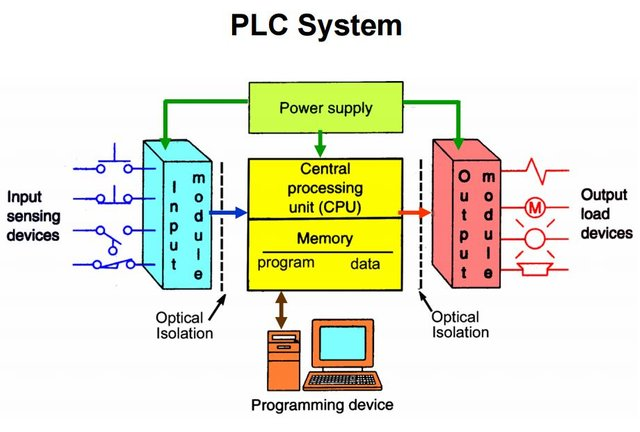
\includegraphics[ clip, trim=0.5cm 0.5cm 0.5cm 0.5cm, width=0.70\textwidth]{./images/plc.JPG}\\
	\quelle\url{https://instrumentationforum.com/t/architecture-of-plc/7059} 
	\caption{Blockdiagramm SPS}
	\label{fig:plcFigure}
\end{figure}

%\subsection{Konzept?}
\subsection{Ausgangssituation} 

Als Vorbild für dieses Projekt dient die Kleinsteuerung Easy vom Hersteller Eaton. Das Einstiegsmodell bietet hier acht Eingänge und vier Ausgänge. Das Logikprogramm, welches die Eingänge der Steuerung logisch mit den Ausgängen verbindet wird hier, auf einem kleinen Display, direkt am Gerät erstellt. Dabei stehen neben den physikalischen Ein- und Ausgängen auch Zeitfunktionen oder Zählerbausteine zur Verfügung. *Erweiterbar* Im Programmiermodus wird links einen Pluspol und rechts einen Minuspol Symbolisiert. Der anzusteuernde Ausgang, welcher obligatorisch ist, steht dabei stets ganz rechts. Der Strompfad kann nunmehr bis zum Pluspol durch gezeichnet werden, oder aber durch Sensoren unterbrochen und verzweigt werden. Aus diesem Schaltplan werden dann die booleschen Gleichungen gewonnen, die die Steuerung im Betrieb durchläuft um die Werte der Ausgänge zu bestimmen.

\begin{figure}[htbp]
	\centering
	\includegraphics[page=2, clip, trim=2.5cm 20cm 6.9cm 2.5cm, width=1.00\textwidth]{./code/GartenEasy.pdf}
	\caption{Programm einer Easy Kleinsteuerng}
	\label{fig:easyprogram}
\end{figure}

\subsubsection{Bedienoberfläche} 
Eine ähnliche Vorgehensweise ist auch in diesem Projekt geplant. Da der Raspberry Pi Netzwerkfähig ist, wurde jedoch anstatt einem Display am Gerät eine Bedienoberfläche gewählt, welche im Internetbrowser bedienbar ist. Als Basis für die Programmieroberfläche, wurde das Projekt CircuitVerse *REF* herangezogen. Hierbei handelt es sich um einen Logiksimulator, in welchem komplexe Logikschaltungen durch Drag\&Drop erstellt werden können. Das Quelloffene Projekt ist auf GitHub *REF* verfügbar und dank  der MIT *REF* Lizenz zur Erweiterung und Modifikation freigegeben. Dabei musste das Projekt vor allem durch eine Funktion ergänzt werden, um die Erstellte Logik in einem Format zu Exportieren, welche vom Backend verstanden wird. Weiterhin musste die zur Verfügung stehenden Ein- und Ausgänge dahingehend modifiziert werden, dass nur Schaltungen erstellt werden können, die auch vom Backend verstanden werden. 
Im Vorbild kann der Schaltplan auch Laufzeitinformationen wiedergeben. So wird ein (symbolisch) unter Spannung stehender Zweig als breite Linie dargestellt, während unbestromte zweige schmal gezeichnet werden. Dies Laufzeitinformationen sollen in dieser Bachelorarbeit ebenfalls dargestellt werden.
\subsubsection{Backend} 
Als Schnittstelle zwischen Hardware und Bedienoberfläche wird eine Software eingesetzt, die das vom Benutzer erstellte Logikprogramm kontinuierlich durchläuft, und somit sicherstellt, das eine Änderung an einem Eingang, der Ablauf eines Timers etc. die Werte der davon abhängigen Ausgänge entsprechend verändert. Wie dies im Vorbild der Easy Kleinsteuerung gelöst wird, bestand kein Einblick.  

\subsubsection{Hardware} 
Wie schon vorab beschrieben, bildet ein Raspberry Pi die Grundlage für dieses Projekt. Dieser bietet von Haus aus einige GPIOs, welche  dazu  verwendet werden können um Sensoren abzufragen oder um Aktoren anzusteuern. Jedoch viel die Entscheidung darauf, eine Erweiterungskarte (HAT) zu diesem Zweck einzusetzen. Dies dient erstmals zum Schutz des Raspberry Pi, zudem bietet das eingesetzte Board jedoch Leuchtdioden an den Ausgängen, sowie Taster an den Eingängen, was das Testen erheblich vereinfacht. Da der Anschluss per SPI erfolgt, können theoretisch mehrere solcher Boards parallel betrieben werden. 

\subsection{Versionsverwaltung}
Da im bisherigen Studium lediglich auf SVN als Versionsverwaltung tiefer eingegangen wurde wobei eine Versionsverwaltung für ein Projekt dieser Größe als notwendig erachtet wurde, fiel der Gedanke auf GIT. Git ist eine dezentrale Versionsverwaltung, die Notwendigkeit für einen Versionierungsserver entfällt hierdurch. Jedoch ist es in Git möglich ein- oder mehrere sogenannte Remotes hinzuzufügen. Das sind entfernte Git-Repositorys die mit dem lokalen Repository synchronisiert werden können. In der Praxis wird Git häufig eingesetzt, weshalb sich diese Bachelorarbeit als Einarbeitung anbot. Zunächst wurde ein lokales Git Repository erstellt, welches in Folge mit einem Remote-Repository auf GitHub verbunden wurde. Angedacht war ein Development-Branch und jeweils ein Feature Branch welcher nach Vollendung des entsprechenden Features in den Development Branch zurückgeführt werden soll. Darüber hinaus, soll ein Tagging erfolgen. Dabei soll für jeden Zeitbalken *WORD* im, in der vorhergehenden Projektplanung erstellten Gantt Diagramm, ein Tag erstellt werden. 

\subsection{Entwicklungsumgebung}
Ein Problem dass dieses Projekt bietet ist, dass nicht direkt auf dem Zielsystem entwickelt wird. Das hat zur Folge, dass das Programm entweder auf dem Entwicklungssystem Crosskompiliert werden muss, oder die Quelldateien auf das Zielsystem kopiert werden müssen um sie dort zu kompilieren. Da das Aufsetzen eines Crosskompilers inklusive der dazu nötigen Toolchain als zu Aufwändig erachtet wurde, blieb nur der Weg das Projekt direkt auf dem Zielsystem zu übersetzen. Um sich die Arbeit zu erleichtern wurde nach einer Entwicklungsumgebung recherchiert, die ein Übersetzen über eine SSH Verbindung zulässt. NetBeans bietet diese an, dabei wird entweder das gesamte Projekt beim Übersetzen per SSH auf das Zielsystem übertragen und dort übersetzt, oder es kann ein Mountpunkt definiert werden, an dem eine Systemfreigabe eingehängt ist (z.B. Samba-Freigabe). Im Laufe des Projektes wurde eigens dafür ein Samba Server auf dem Zielsystem installiert. Von nun an konnte also in der Entwicklungsumgebung direkt auf den Dateien des Raspberry Pi gearbeitet werden, wobei per Tastendruck eine SSH Verbindung aufgebaut wird um auf dem Zielsystem \chphl{make} auszuführen. Dabei werden sämtliche Comiler Ausgaben in einem Fenster angezeigt. Auch Debugging ist auf diesem Wege möglich.

\subsection{C++ Library LibPiFace}
Wie im vorhergenenden Abschnitt *REF* beschrieben, bildet die Erweiterungskarte PiFace Digital 2 *REF* die Grundlage für diese Bachelorarbeit. Im Lieferumfang befindet sich eine in C geschriebene Library inklusive eines Lauffähigen Tests, welche ebenfalls auf GitHub unter https://github.com/piface/libpifacedigital zu finden ist. Diese Library stützt sich wiederrum auf die Library https://github.com/piface/libmcp23s17 welche den verbauten SoC über SPI anspricht. Im Laufe der Arbeiten fiel jedoch auf, dass die C Library nicht alle benötigten Funktionen enthielt. Da der Quellcode vorlag, und die Lizensierung Veränderungen am Quellcode zulässt, lag die Überlegung nahe die benötigten Funktionen direkt in der Library zu ergänzen anstatt sie im eigentlichen Projekt unterzubringen. Weiterhin schien es auch ein erstrebenswertes Lernziel zu sein, das Erstellen und Übersetzen von statisch bzw. dynamisch gelinkten Bibliotheken kennenzulernen. Zuletzt schien es schlichtweg die Sauberste Lösung zu sein. Zunächst wurde angenommen, dass sich auch mehrere Hardwaremodule per SPI mit einem einzelnen Rasperry Pi verbinden lassen. Dies ist technisch auch möglich, so bieten die eingesetzten Boards die Möglichkeit über einen Jumper eine Hardwareadresse einzustellen. Der Hersteller bot auch die passende Hardware an, um mehrere Boards mit einem Rasperry Pi zu verbinden. Jedoch wurden diese scheinbar mangels Nachfrage aus dem Sortiment genommen. Obwohl eine Bastellösung es immer noch ermöglichen würde, ist der Aufwand hierfür sehr hoch und scheint unwirtschaftlich. Leider wurde bis zu dieser Erkentniss schon einiges an Energie darin investiert, mehrere Boards zu unterstüzen. Dies ist auch der Grund wieso ein Objektorientierter Ansatz in C++ gewählt wurde - eine Instanz für jedes Harwaremodul. Ein weiterer Grund war, dass die Anwendung ohne Caching nicht performant genug war. Das heißt die zeitliche Lücke zwischen einer Änderung an einem Eingang bis zu dessen Auswirkung am Ausgang war deutlich spürbar. Dafür wurden Methoden vorgesehen, um das Caching ein un auszuschalten - bei eingeschaltetem Caching verändern die Methoden um Bytes und Bits zu schreiben, lediglich den Wert einer Instanzvariable. Derzeit muss das leeren des Chaces explizit mittels Aufruf der Methode \textit{flush()} erfolgen. Über ein Automatisches verfahren wurde nachgedacht, jedoch erwies sich der manuelle Aufruf als einfacher. 

    
\clearpage


\newcommand{\pthUmsetzung}{\pthChps/umsetzung}
\section{Umsetzung}
\label{chp:Umsetzung}


\renewcommand{\pthImg}{\pthVerlauf/img}
\renewcommand{\pthDoc}{\pthVerlauf/doc}



Beschreibung, Begründung



\newcommand{\pthAuswertung}{\pthChps/auswertung}
\section{Auswertung}
\label{chp:Auswertung}
\section{Übersicht Gesamtsystem}\label{kap:ausw}
 \subsection{Inbetriebnahme}
 \subsubsection{Hardware Voraussetzungen}
 Voraussetzung für den Betrieb ist ein Raspberry Pi 2 oder 3. Außerdem ist eine Erweiterungsplatine \chphl{PiFace Digital2 \cite{URL:PiFaceDigital2}} erforderlich. Diese muss vor dem ersten Start auf die GPIO-Kontakte des Raspberry Pi aufgesteckt werden. Eine Funktion ohne das Hardwaremodul ist Grundsätzlich möglich, jedoch scheint ein Betrieb ohne Hardwareschnittstelle ohne Sinn. Die Software ist so konzipiert, dass auch andere Hardware-Module denkbar sind, eine Implementierung hierfür fehlt jedoch bislang.     
 \subsubsection{Software Voraussetzungen}
 Für den Betrieb wird ein Linux Betriebssystem vorausgesetzt. Hierfür kann das angepasstes Raspbian \cite{URL:Raspian} Image genutzt werden, welches auf der beigelegten DVD zu finden. Falls auf der SD Karte bereits ein Linux Betriebssystem installiert ist, kann das Arbeitsverzeichnis des Projekts auch einfach auf den Raspberry Pi übertragen werden. Ein Git Auszug hiervon ist ebenfalls auf der beigelegten DVD. Sollte die Wahl der Distribution auf eine andere als Raspbian Strech \cite{URL:Raspian} fallen, so muss das Projekt aus den Quellen übersetzt werden. In jedem Fall ist es nötig dass SPI aktiviert wird. Dies geschieht am einfachsten über das Raspberry Pi Konfigurationsprogramm.  \texttt{sudo raspi-config} siehe \cite{URL:EnableSPI}.  
 \subsubsection{Kompilieren des Projekts}
 Ein kompilieren des Projekts ist nur erforderlich, wenn das Projekt auf einem anderen Betriebssystem als Raspbian Strech \cite{URL:Raspian} verwendet werden soll, oder wenn Änderungen am Quellcode vorgenommen werden sollen. Dafür muss zunächst eine SSH Verbindung zum System herstellt werden. Das Projekt sollte daraufhin auf das System übertragen werden. Die empfohlene Vorgehensweise hierfür ist, das GIT Repository über eine aktive Internetverbindung auf den Rasperry Pi zu klonen. \texttt{git clone https://github.com/dajuly20/ControlPi}. Um dann alle Abhängigkeiten automatisch zu installieren, kann das nachfolgend genannte Installationsscript verwendet werden: \texttt{./start\_pull\_and\_build.sh}. Sollte keine Internetverbindung bestehen, können die auf der DVD mitgelieferten Bibliotheken auch manuell installiert werden. 
 Eine Liste der benötigen Abhängigkeiten findet sich im \nameref{chp:anhang} in \autoref{chp:anhang}.  
 \subsubsection{Inbetriebnahme unter Raspbian Strech}
 Sollte auf dem Raspberry Pi bereits ein Version von Raspbian in der Version Strech installiert sein, so genügt es den Projektordner auf den Raspberry Pi zu übertragen. Hierfür dient entweder der Ordner \texttt{ControlPi} auf der beigelegten DVD, oder das GIT Repository des Projekts, welches mittels  \texttt{git clone https://github.com/dajuly20/ControlPi} auf den Raspberry Pi übertragen werden kann. Um sicherzustellen dass es sich um die aktuellste Version handelt, sollte das Projekt mit \texttt{git pull} auf den neusten Stand gebracht werden. Daraufhin kann mit \texttt{./start\_manual.sh} die Funktion überprüft werden. Dabei sollte der Benutzer in den Gruppen \texttt{spi} sowie \texttt{gpio} sein. Letztlich sollte das Projekt als Systemservice eingerichtet werden. Hierfür ist das Script \texttt{./start\_as\_service.sh} dienlich. Es wird hier neben dem eigenen Systemservice auch ein Apache2 Webserver mit in Betrieb genommen.
 
 \subsection{Inbetriebnahme mit Systemabbild}
 Auch befindet sich ein vollständiges Systemabbild \cite{URL:Image} auf der beigelegten DVD. Dieses sollte zunächst mit \texttt{tar -xvzf ControlPi-Raspbian-Strech.tar.gz} entpackt werden. Die enthaltene \texttt{.img} Datei belegt ca. 7,3 GB. Eine Speicherkarte sollte also mindestens 8 GB besser jedoch 16 GB Platz bieten. Das Systemabbild kann mit \texttt{sudo dd if=ControlPi-Raspbian-Strech.img of=/dev/<XXX> bs=4M status=progress}, oder unter Windows mit einem entsprechenden Tool \cite{URL:Win32DiskImager} auf eine Speicherkarte übertragen werden. Nach erfolgreichem Start sollte eine der LEDs auf der PiFace Erweiterungskarte dauerhaft blinken.  
 
 \subsubsection{Ermittlung der IP - Adresse}\label{chp:ausw:ip}
 Nachdem der Systemservice läuft, muss nun ermittelt werden wie ein Zugriff auf die Weboberfläche erfolgen kann. Wenn der Raspberry Pi in ein bestehendes Netzwerk integriert wird, kann dies in der Oberfläche des verwendeten Internetrouters nachgesehen werden. Sofern dieser dies unterstützt, kann auch der Hostname des Raspberry Pi für den Zugriff verwendet werden. Der Hostname im mitgelieferten Raspbian-Image lautet \texttt{ControlPi3}. Der Standard bei einem offiziellen Raspbian Image ist \texttt{raspberrypi}. Sollte kein Zugriff auf den Internetrouter bestehen oder eine Ermittlung der IP Adresse aus sonstigen gründen nicht möglich ist, kann ein Portscan durchgeführt werden. Die Steuerung öffnet in der Standartkonfiguration die Ports 80 für HTTP, den Port 443 für HTTPS bzw. SSL und den Port 22 für SSH Zugriffe. Angenommen eigene IP Adresse (Ermittlung durch \texttt{ifconfig}) wäre 192.168.8.5 mit der Subnetzmaske 255.255.255.0 so wäre der Aufruf \texttt{nmap -p 22,80,443 192.168.8.0/24}. Sollten mehrere gefundene Geräte diese Ports als offen anzeigen, so sollten die IP Adressen dieser Geräte nacheinander im Webbrowser als URL eingetragen werden um zu überprüfen bei welcher es sich um die richtige handelt.   
 
 \subsection{Funktionstest}
 \subsubsection{Testen der Betriebsbereitschaft}
 Im Auslieferungszustand ist ein zu Testzwecken bereits ein Steuerungsprogramm enthalten. Dieses lässt die LED an Ausgang 6 durch einen sich selbst aufrufenden Timer blinken. Zudem ist in diesem Testprogramm den Ausgängen \texttt{0} sowie \texttt{1} der Wert der Eingänge \texttt{0} beziehungsweise \texttt{1} zugewiesen. Ein Drücken der in \autoref{img:PiFaceDigital2} gezeigten Taster S0 oder S1 sollte also ein Leuten der entsprechenden LED zur Folge haben. Wie auch bei den Tastern, werden die LEDs von rechts nach links durchnummeriert und sind den jeweiligen Ausgängen örtlich zugeordnet. Da an den Ausgängen \texttt{0} und \texttt{1} zudem Relais angeschaltet sind, sollte sich ein Zustandswechsel auf einem dieser Ausgängen außerdem in Form eines Klickgeräusches akustisch bemerkbar machen. 

 
 \begin{figure}[H]
 	\begin{center}
 		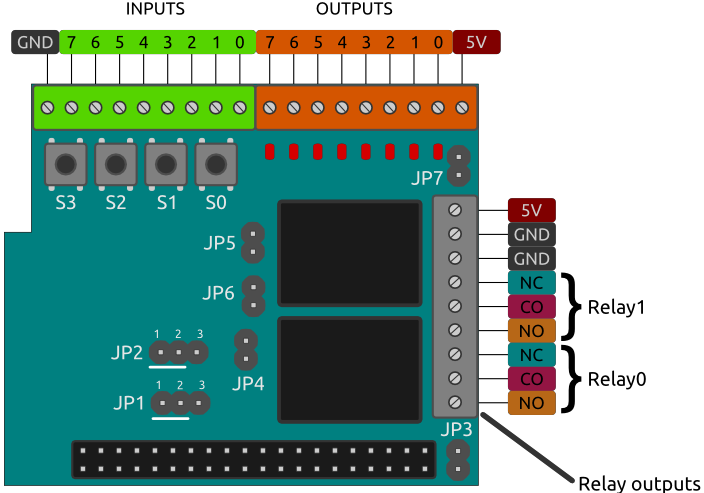
\includegraphics[width=0.95\textwidth]{./images/pifacedigital2_diagram.png}
 		\caption[Darstellung eines PiFace Digital 2]{Darstellung eines PiFace Digital 2 \cite{URL:Pfd}}
 		\label{img:PiFaceDigital2}
 	\end{center} 
 \end{figure}	

 \subsubsection{Aufruf der Weboberfläche}\label{chp:FrontendUebersicht}
Ist der Hostname oder die IP Adresse des Raspberry Pi ermittelt (siehe Abschnitt \ref{chp:ausw:ip} \nameref{chp:ausw:ip}), kann dieser im Internetbrowser aufgerufen werden. Bei Verwendung des beigelegten Raspbian Images wäre der Aufruf \texttt{http://ControlPi3}. \autoref{img:FrontendUebersicht} zeigt die Übersichtsseite der Steuerung. In der Mitte befindet sich eine Abbildung vom aktuell verwendeten Steuerungsprogramm, während an den Seiten die Zustände ein und Ausgänge angezeigt werden. Die Drop-Down Menüs oberhalb, ermöglichen es die gewünschte Ein- bzw. Ausgangsentität auszuwählen. Handelt es sich bei der ausgewählten Entität um einen Eingang, so wird anstelle einer LED ein Taste eingeblendet. Der Zustand kann dann, bei entsprechender Berechtigung (siehe \chpref{chp:ums:websock:auth} ), durch anklicken verändert werden.  

 \begin{figure}[H]
	\begin{center}
		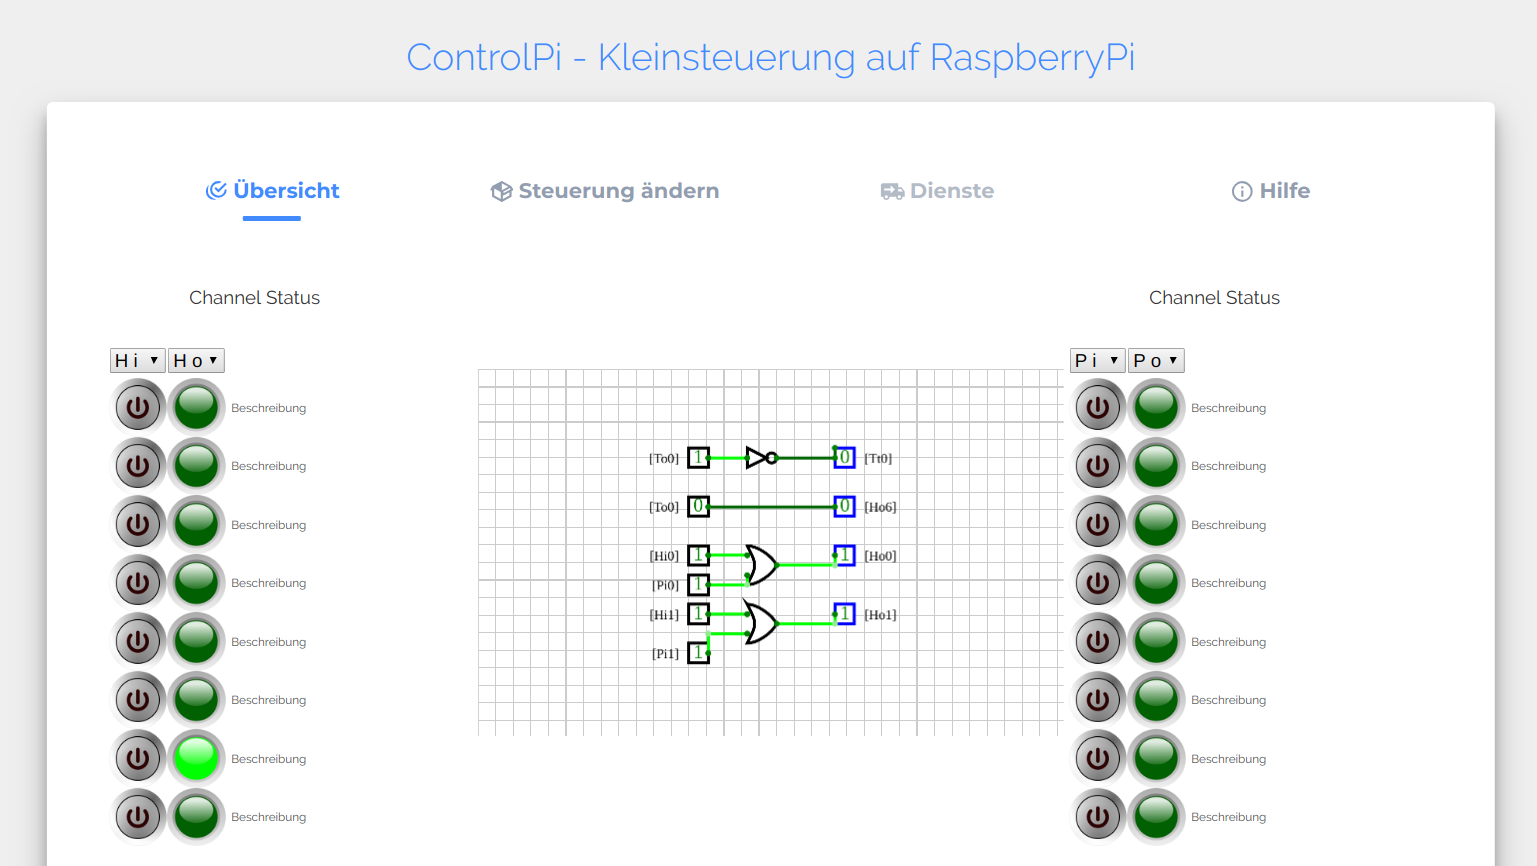
\includegraphics[width=0.95\textwidth]{./images/FrontendUebersicht.png}
		\caption{Darstellung Frontend Übersicht}
		\label{img:FrontendUebersicht}
	\end{center} 
\end{figure}

\subsubsection{Erstellen eines Steuerungsprogramms}

Um ein Steuerungsprogramm zu erstellen, muss zunächst der Tab \texttt{Steuerung ändern} angewählt werden. Nun erscheint der in \autoref{img:FrontendAenderung} abgebildete Logik-Editor CicuitVerse \cite{URL:CircuitVerse}. Sollte die vorhandene Logikschaltung nicht sofort sichtbar sein, muss die Zeichenfläche zuerst durch klicken auf das Fadenkreuz-Symbol in den Mittelpunkt gerückt werden. Soll nun eine komplett neue Schaltung gezeichnet werden, kann die Zeichenfläche durch den Unterpunkt \texttt{Clear Project} im Drop-Down Menü \texttt{Project} bereinigt werden. Alle verfügbaren Bauteile befinden sich im Bauteil-Menü auf der linken Seite. Dieses ist in die Kategorien \texttt{Input} \texttt{Output} und \texttt{Gates} unterteilt, welche sich durch anklicken aufklappen lassen. Möchte man ein Bauteil auf die Zeichenfläche schieben, so muss dieses angeklickt und der Cursor auf die Zeichenfläche bewegt werden. Ein erneutes Klicken lässt das Bauteil an der gewählten Position fallen. Die Bauteile werden schließlich mittels Drag \& Drop mit einander Verbunden. Werden Timerbausteine angeklickt, so  lassen  sich dessen Einschalt und Ausschalt- Verzögerungszeiten im Menü \texttt{Properties} einstellen. Es gilt zu beachten, dass Ausgänge jeweils nur einmal vorkommen dürfen. Gibt es mehrere Möglichkeiten in denen ein Ausgang aktiv werden soll, empfiehlt sich die Verwendung eines Und- bzw. Oder- Gatters. Nach Vollendung des Steuerungsprogramms, kann die Steuerung mit dem Menüpunkt \texttt{Save \& Export}, welcher sich im Menü \texttt{Project} befindet, übernommen und getestet werden. Eine Überprüfung auf Richtigkeit des Steuerungsprogramms erfolgt nicht. Deshalb sollte der Info-Kasten \texttt{Backend Status} im Auge behalten werden. Falls ein Fehler mit dem Steuerungsprogramm auftritt, wird dieser dort angezeigt. 
	

 \begin{figure}[H]
	\begin{center}
		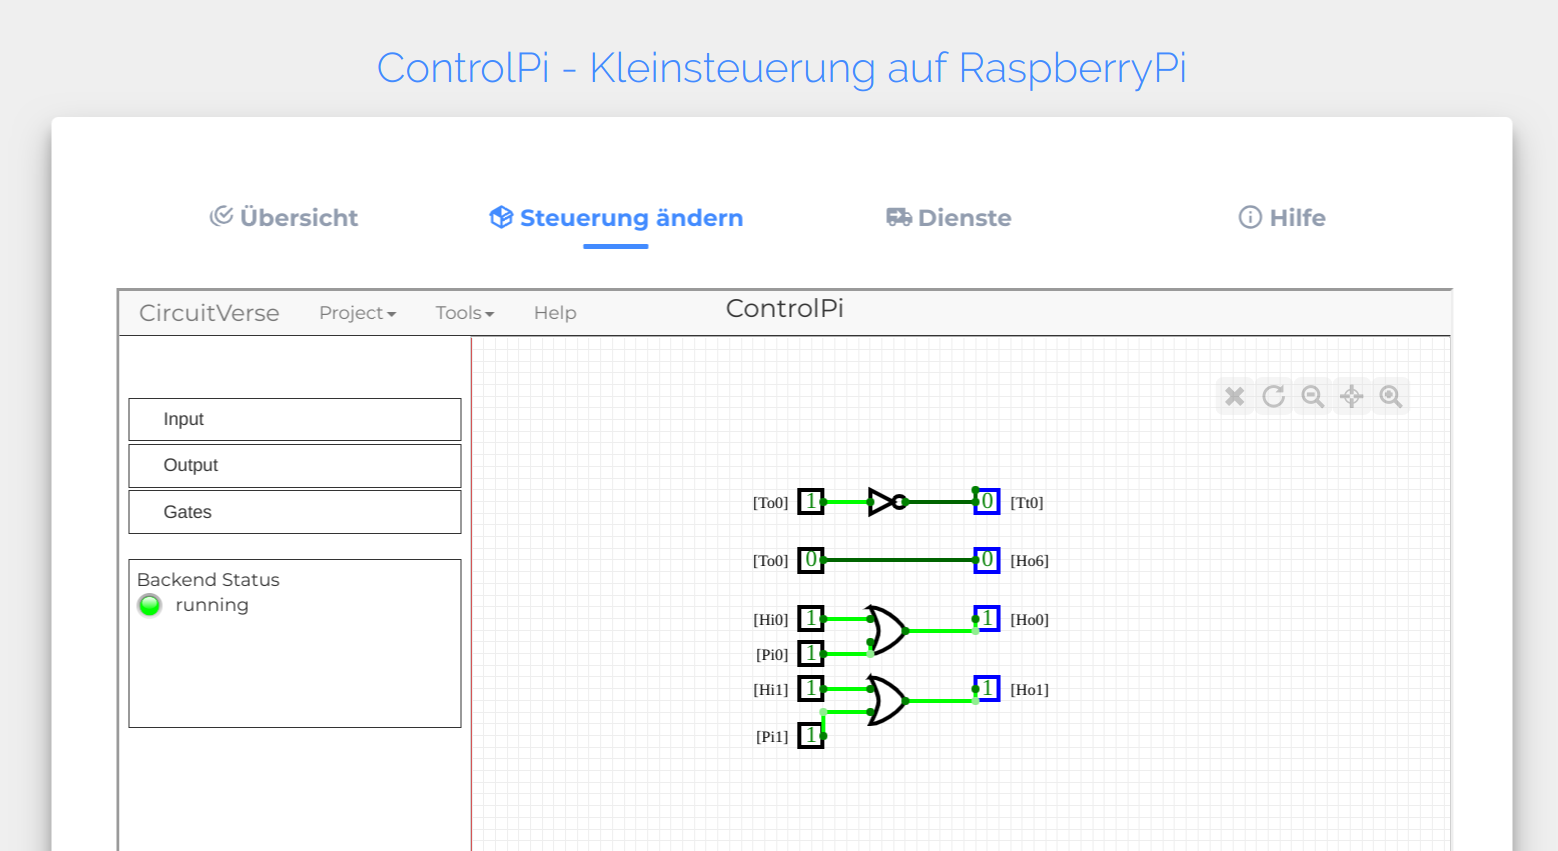
\includegraphics[width=0.95\textwidth]{./images/FrontendAendern.png}
		\caption{Darstellung Logik Editor}
		\label{img:FrontendAenderung}
	\end{center} 
\end{figure}	

\subsection{Langzeittest}
Um zu Testen wie sich die Steuerung längerfristig verhält wurde ein Timerbaustein verwendet, welcher sich selbst nach Ablauf schaltet und somit oszilliert. Als Testzeitraum wurde 48 Stunden gewählt. Dabei ließ sich feststellen, dass die Steuerung auch nach Ablauf dieser Zeit ohne Fehler weiterhin blinkte. Eine Recherche nach Neustarts des Systemdienstes blieb ebenfalls ohne Treffer.    

 \subsection{Bugs}
 Zum derzeitigen Stand sind noch einige Probleme enthalten auf die nachfolgend eingegangen wird. Als erstes sei hier zu nennen, dass die Reihenfolge in welcher das Backend über die Zeilen des erzeugten Steuerungsprogramms Iteriert unter bestimmten Voraussetzung Probleme bereitet. So wird der Wert eines Ausgangs unter noch nicht näher bekannten Umständen erst mit der nächsten Iteration des Logikprogramms übernommen. Dies könnte durch generelles doppeltes iterieren behoben werden, was allerdings die Performance vermindert. Der Logikeditor in der Benutzeroberfläche hat ebenfalls ein Darstellungsproblem welches bislang noch nicht behoben werden konnte. Beim Aufruf wird die bereits vorhandene Logikschaltung nicht Automatisch zentriert, sondern ist beinahe unsichtbar in der oberen linken Ecke der Zeichenfläche. Ein klicken auf das Fadenkreuz-Symbol bringt hier Abhilfe.  
 
 \subsection{Fazit}
 Das Projekt teilte sich wesentlich in zwei Teile. Das Backend ist einen Teil, welcher sich auf einer sehr Hardwarenahen Ebene abspielte. Die Benutzeroberfläche hingegen, ist sehr nahe am Benutzer. Damit spiegelte dieses Projekt viele Nuancen der Technischen Informatik wieder. Die meiste Arbeit entfiel dabei in die Programmierung des Backend, dass in mehrere parallele Handlungsstränge aufgeteilt ist, welche synchronisiert werden wollen. Auch das arbeiten mit C++ Bibliotheken und das Kompilieren brachte einige Herausforderungen mit sich. Die Anbindung der Benutzeroberfläche beleuchteten eine relativ junge Technologie der modernen Webentwicklung. Auch das Anpassen des Logik Editors und die damit verbundene Einarbeitung in ein fremdes Open-Source Projekt machten dieses Projekt sehr lehrreich. Zuletzt boten sich auch die Gelegenheit zu erproben wie eine Software durch Systemabbilder oder Git verteilt werden kann, und wie man diese mit \LaTeX\ so dokumentiert, dass möglichst alle Aspekte beleuchtet werden und die  Arbeit unkompliziert weitergeführt werden kann.
 
 \subsection{Ausblick}
 Die Steuerung funktioniert in den meisten Fällen ohne Probleme, ist jedoch noch nicht über ein frühes Betastadium hinaus. Es bedarf nun Feldtests um weitere Bugs in der Software aufzuspüren. Außerdem sind noch einige Funktionserweiterungen Denkbar. Zuerst anzuführen wäre hier die Kopplung zweier Geräte. Die Grundvoraussetzungen hierfür sind durch die Implementierung  von Websockets bereits geschaffen. Entweder müsste hier eine Mittelschicht geschrieben werden, welche die zwei Websocket Server auf den beiden Geräten miteinander kommunizieren lässt. Etwas eleganter jedoch wäre die Implementierung eines Websocket Clients in das Backend. Mit einer angepassten Konfigurationsdatei könnte das Backend sich so zu einem anderen Gerät verbinden um dessen Virtuelle Ein und Ausgänge auch am lokalen Gerät nutzbar zu machen. Websockets haben durch die persistente Verbindung sehr gutes Verhältnis zwischen Overhead und Payload und sollten somit eine recht geringe zeitliche Verzögerung ermöglichen. Die Erfahrung von der Verbindung zwischen Web-Frontend und Backend zeigen kaum merkliche Verzögerungszeiten. Eine weitere Funktion über welche nachgedacht wurde, ist ein anlegen von Unterstromkreisen. Somit könnten zum Beispiel blinker Bausteine oder \texttt{Stromstoßschalter}, das sind Bauteile die ihren Logikzustand durch einen Eingangsimpuls wechseln, realisiert werden. Dabei würde die Implementierung abstrahiert und die Übersichtlichkeit erhöht. Ebenfalls denkbar wäre die Zusammenfassung der Timer Ein- und Ausgänge in ein einziges Bauteil. Die Umsetzung beim Export könnte hierbei beibehalten werden, jedoch könnten die Timer Bausteine dann zwischengeschaltet werden, was deren Einsatz vereinfacht. 
  

 
 
\clearpage



%\newcommand{\pthGeneric}{\pthChps/generic}
%\section{Generic}
%\label{chp:Generic}
%

\renewcommand{\pthImg}{\pthVerlauf/img}
\renewcommand{\pthDoc}{\pthVerlauf/doc}








%\section{Resumé}
%\label{chp:Resume}




%----- %
\newpage
%----- %

\listoffigures
%----- %
\newpage
%----- %
\listoftables

%----- %
\newpage
%----- %
\lstlistoflistings	

 \begin{thebibliography}{999}
  
  \bibitem {ResyncMySqlReplication} Stackoverflow Anleitung zum resynch eines Master-Slave setup \url{https://stackoverflow.com/a/3229580/3142746}
  \bibitem {DatenblattIC} Datenblatt Quelle \url{http://pdf1.alldatasheet.com/datasheet-pdf/view/28193/TI/SN75175.html} \textit{Abruf: 30.05.2018 13:00}
  \end{thebibliography}

\end{document}